%---- Sample WMSU BSMATH BEAMER template ------
%---- Begin editing after PREAMBLE END at line 77------
%---- Created by: Christle Jude L. Maquilan - April 2022 --
%---- @jmaq03.jm@gmail.com -----

\documentclass[xcolor=dvipsnames,envcountsect]{beamer}

%-------- theme --------
\usetheme{Madrid}

%-------- color --------
\definecolor{peagreen}{RGB}{180,216,45}
\definecolor{darkpastelgreen}{rgb}{0.01, 0.75, 0.24}
\definecolor{pantone339}{RGB}{0, 178, 134}


\usecolortheme[named=pantone339]{structure}
%-------- set color of 'example block' to crimson theme --------
\setbeamercolor{block body example}{bg=white}
\setbeamercolor{block title example}{fg=white, bg=red!80!black}

%-------- font --------
\setbeamerfont{structure}{family=\rmfamily,series=\bfseries}
\usefonttheme[stillsansseriftext]{structurebold}
\setbeamerfont{section in head/foot}{size=\tiny}

%-------- misc structure --------
\useoutertheme[footline=authortitle,subsection=false]{miniframes}
\useinnertheme{rounded}
\addtobeamertemplate{block begin}{}{\justifying}
\newtheorem{remark}[theorem]{Remark}
\renewcommand{\indent}{\hspace*{2em}}
\setbeamertemplate{theorems}[numbered]
\setbeamertemplate{caption}[numbered]
\usepackage[justification=centering]{caption}
\renewcommand{\qedsymbol}{$\blacksquare$}

%-------- packages to be used -------
\usepackage{amsmath,amsfonts,amssymb,amscd,amsthm}
\usepackage{graphicx,xcolor,comment}
\usepackage{mathrsfs} 
\usepackage{multirow}
\usepackage{array}
\usepackage{hyperref}
\usepackage{multicol}
\usepackage{ragged2e}
\usepackage{caption}
\usepackage[english]{babel}
\usepackage{rotating}
\usepackage{enumerate}
\usepackage{tikz}
\usepackage{bm}
\usepackage{csquotes}
\usepackage{gensymb,textcomp,mathcomp}

\graphicspath{{Figures}}

\newcommand{\flushdown}{\vskip0pt plus 1filll}

%-------- for bibliography -----------------
\usepackage{biblatex}
\setbeamertemplate{bibliography item}{\insertbiblabel}
\addbibresource{main2_references.bib}
\setbeamertemplate{frametitle continuation}{\frametitle{\color{white}List of References}}
% remove section headline
\setbeamertemplate{headline}{}

\title[What is in my Sample?]{What is in my Sample? – Challenges and Approaches for Unveiling the Hidden Diversity in Plankton Samples}

\author [Hoffmann, Marie]{\textbf{Marie Hoffmann (MSc Computer Science)}}

\institute[Western Mindanao State University] {\emph{Advisers: }\textbf{Prof. Knut Reinert, Prof. Michael T. Monaghan}\\[1em]
	Department of Mathematics and Computer Science\\Free University Berlin\\[1em]

\includegraphics[scale=0.06]{./Figures/fu_logo5.png}}

\date[August 23, 2022]{\footnotesize Disputation - \textbf{August 23, 2022}}
%--------- DURATION 20 MIN ------------------

\begin{document}
	
\begin{frame}{\titlepage}\end{frame}
% \begin{frame}{\frametitle{Presentation Outline}\tableofcontents}\end{frame}


%--------- INTRODUCTION ----------------------
\section{Metabarcoding} % Motivation
\subsection{Motivation}
% \begin{frame}\frametitle{Motivation}
\begin{frame}{Motivation: Lake Monitoring Project}
\framesubtitle{Conducted at IGB Berlin}
\begin{figure}
    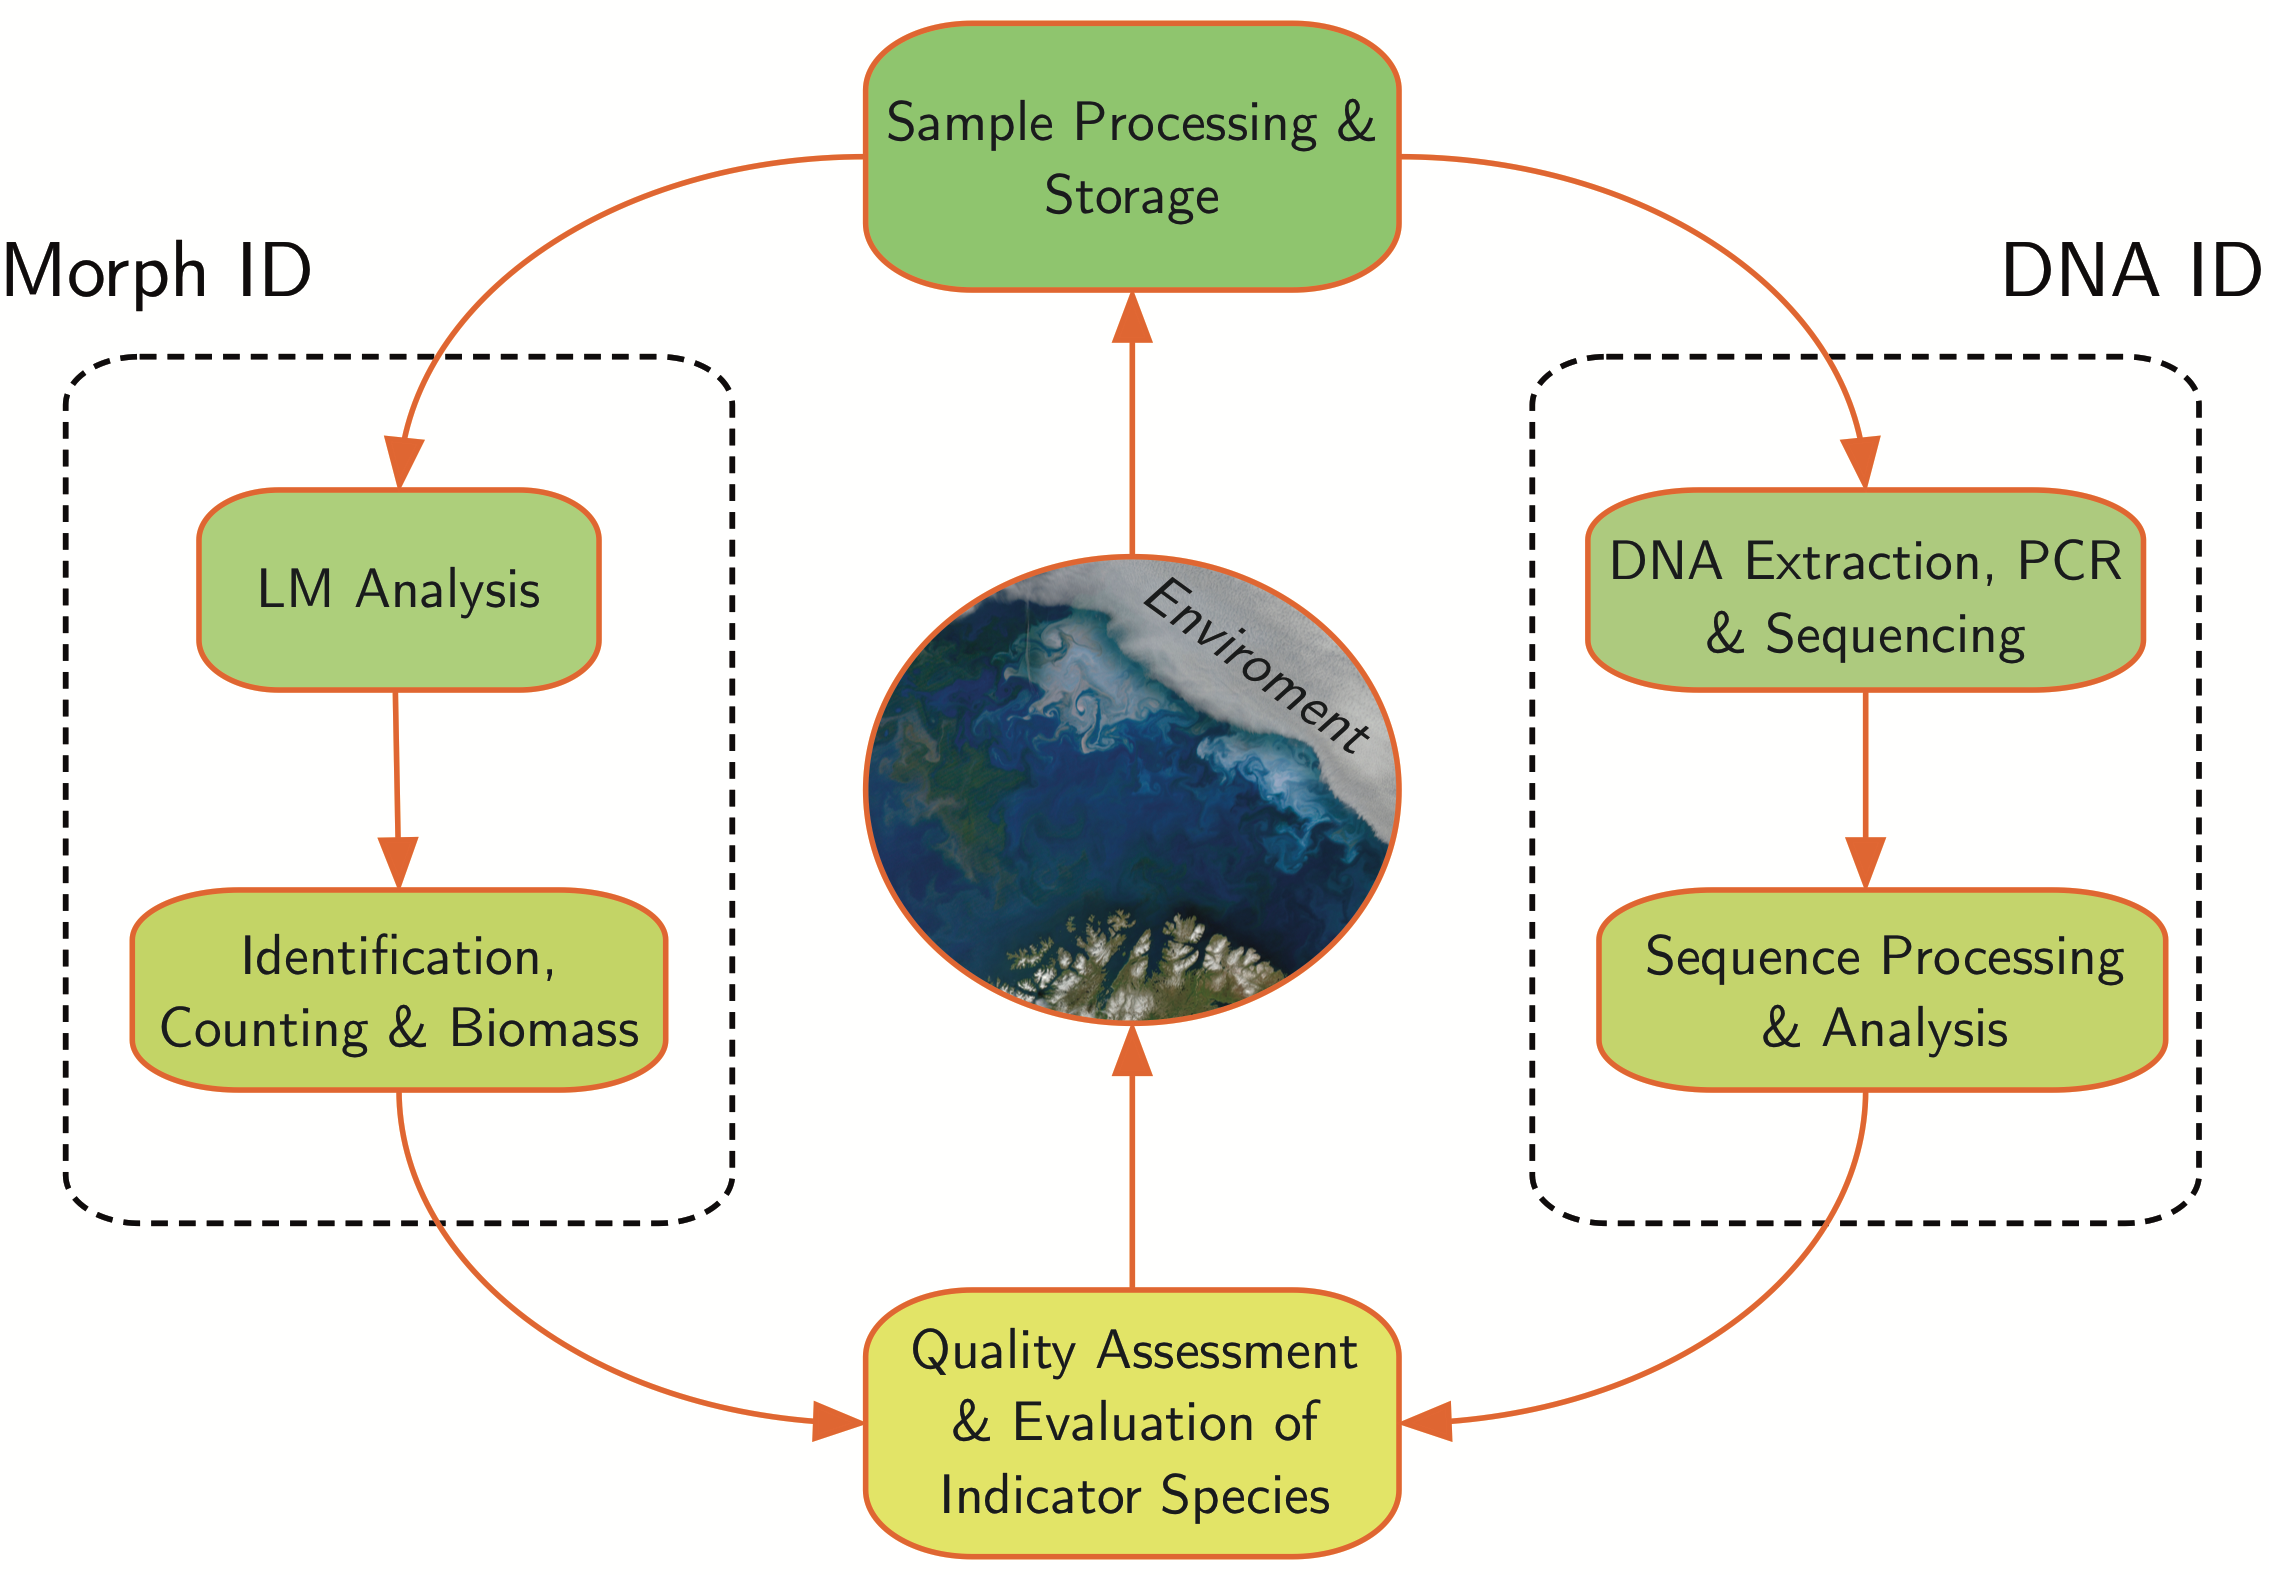
\includegraphics[scale=.6]{sample_processing}
    \caption{Complementing processing pipeline to study dynamics of freshwater samples.}
\end{figure}
\end{frame}

\begin{frame}{Motivation: Lake Monitoring Project}
\framesubtitle{Challenge: Species Diversity I}
\begin{figure}
    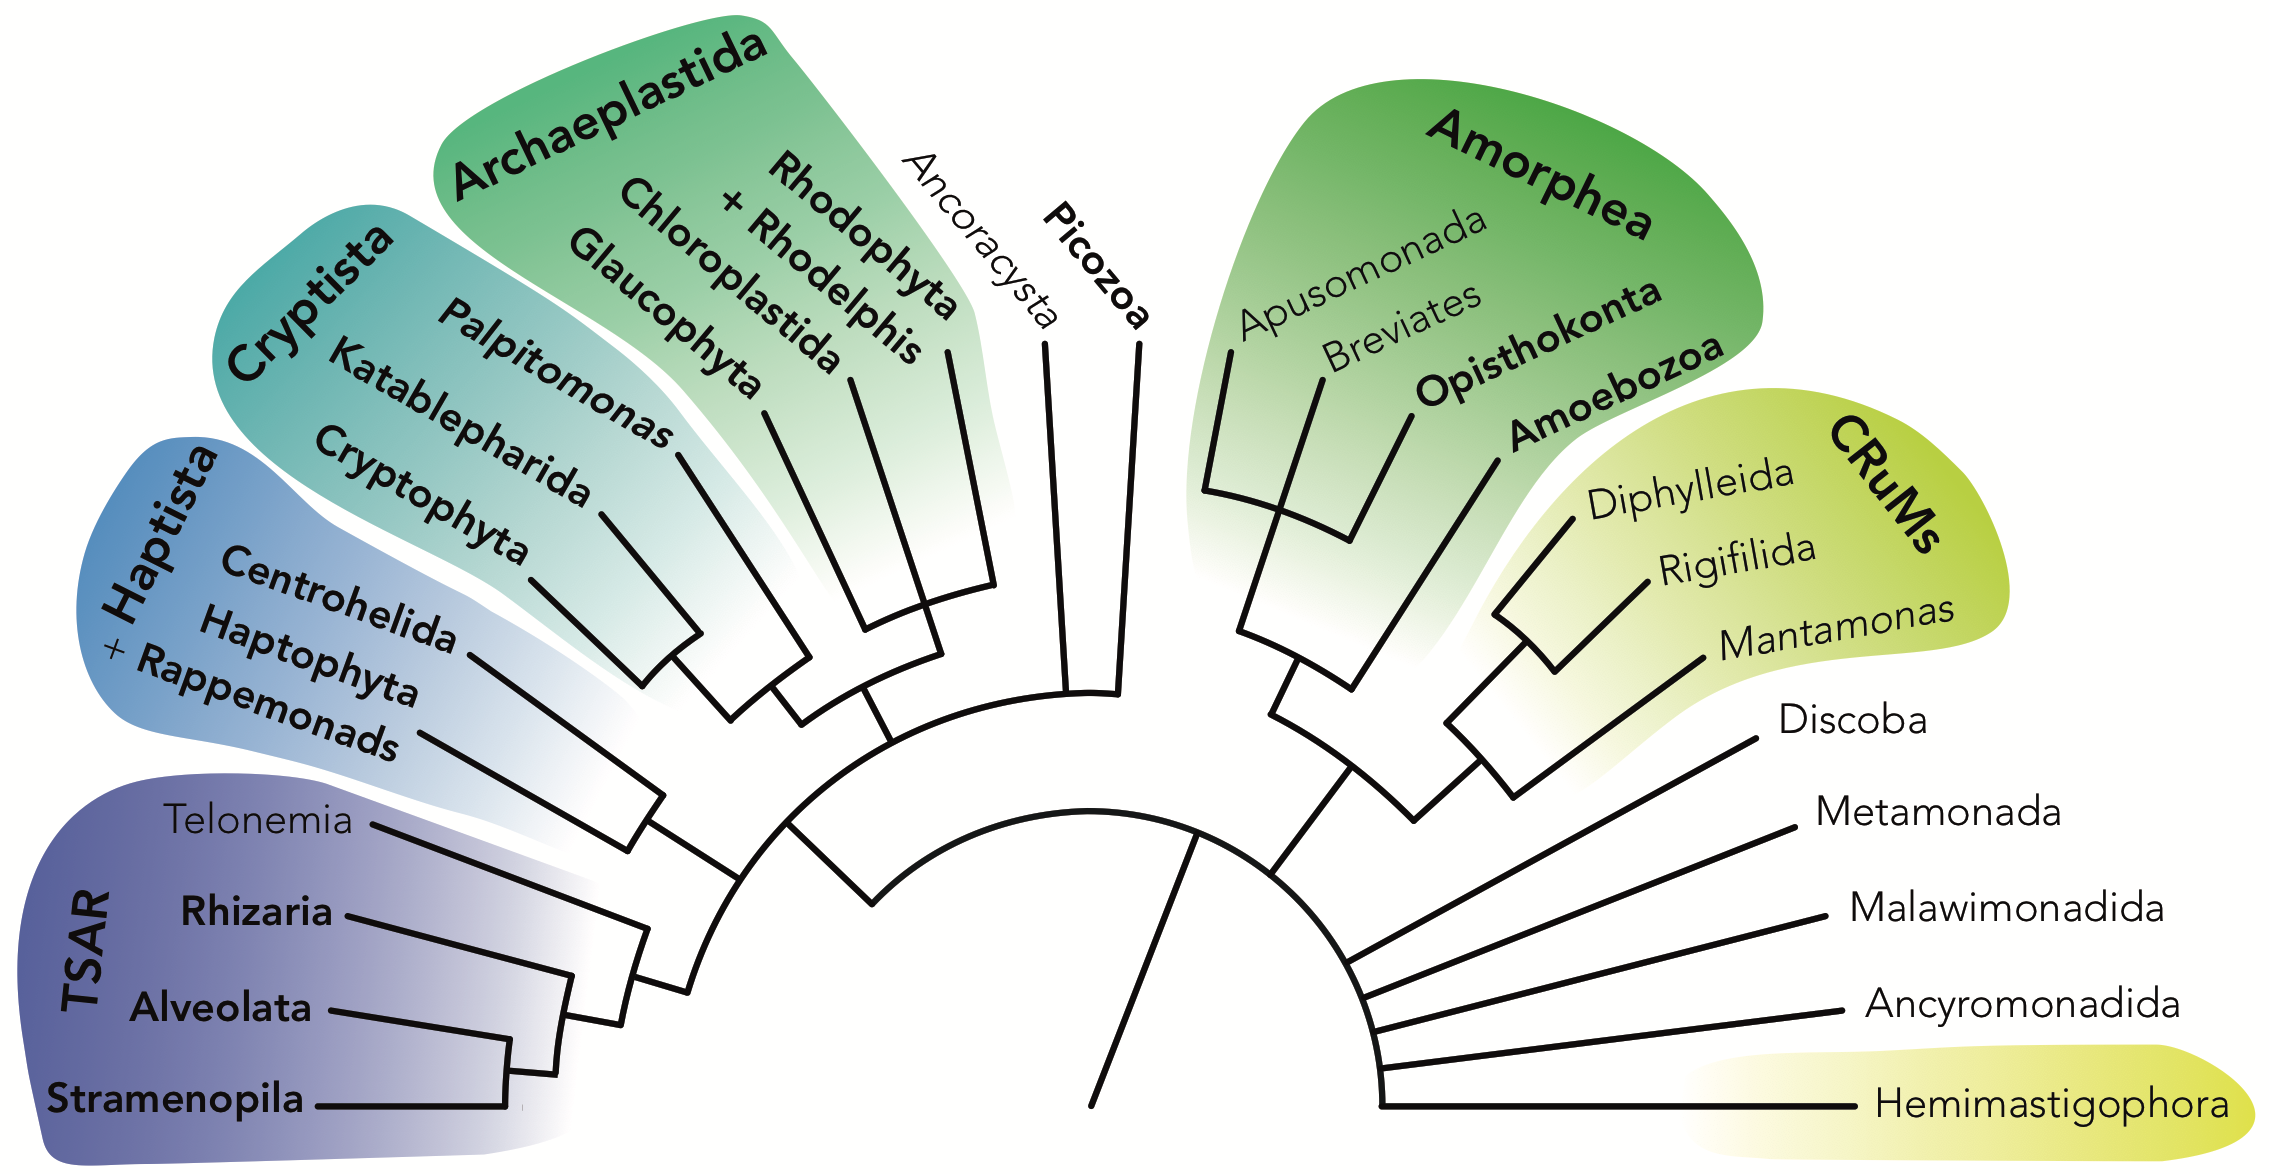
\includegraphics[scale=.6]{eTOL2}
    \caption{Dendrogram of the eukaryote tree of life proposed by \cite{Burki2020}.}
\end{figure}
\end{frame}

% * last point analyzed in Lake Monitoring Study
% * key findings:
% * Thesis 1:
%     * NGS, concretely metabarcoding allows for better presence/absence test of species
%     * binocular reading for now irreplaceable for abundance estimation, description of unknown species, description of malformations
%     * needs to be combined with better in silico methods, e.g., if a species not present, we should be able to rule out the possibility that the applied primers simply would not match
% *  
%     1. Metabarcoding has the potential to identify more clades and nebenher even clades not intended to be monitored (fungi), more clades with higher resolution
%     2. But some clades would remain undetected without the human operator in the loop, e.g., rotifera seen under the microscope, but undetected with three different primer pairs
%     3. Observation of teratological forms (indicators for environmental changes), body size estimation (same) or individual counts can only be done by manual operators 
%         * it is inherently difficult to derive individual counts from DNA reads 
%         * does not scale equally across various species
%         * each PCR unique, biased towards some species


\begin{frame}{Motivation: Lake Monitoring Project}
\framesubtitle{Challenge: Capturing Diversity via NGS}
\begin{enumerate}
     \item Primer Design: taxonomic {\it width} versus {\it depth} % Taxonomic heterogeneity 
    \item Optimization: Missing ground truth % => need to remain sensitive, unbiased
    \item Resolution: Databases are sparse, erroneous, uncurated % partial sequences, rarely complete genomes
    \item Consolidation: No unique, generally accepted taxonomic tree!  % if consulting multiple databases to maximize ID
    % \item Few human experts available (to support complementation of unlabeled sequences)
    \item  PCR: Same difficulties as single organisms DNA analysis: repeats, intra-species variation, ...
\end{enumerate}
\end{frame}


\begin{frame}{Motivation: Lake Monitoring Project}
\framesubtitle{Desiderium for Ongoing Protocol Enhancement}
\begin{enumerate}[I]
    \item Robust {\it de novo} primer discovery and {\it in silico} evaluation % understanding its efficiency
    \begin{itemize}
        \item Automated primer candidate search in uncurated databases % like NCBI’s nt dataset
        % \item Tool required to be
        % \begin{itemize}
            \item Robust to sequencing errors
            % \item mislabeling
            \item Preference for high-frequent proto-primers
        % \end{itemize}
    \end{itemize}
\end{enumerate}
\begin{figure}
    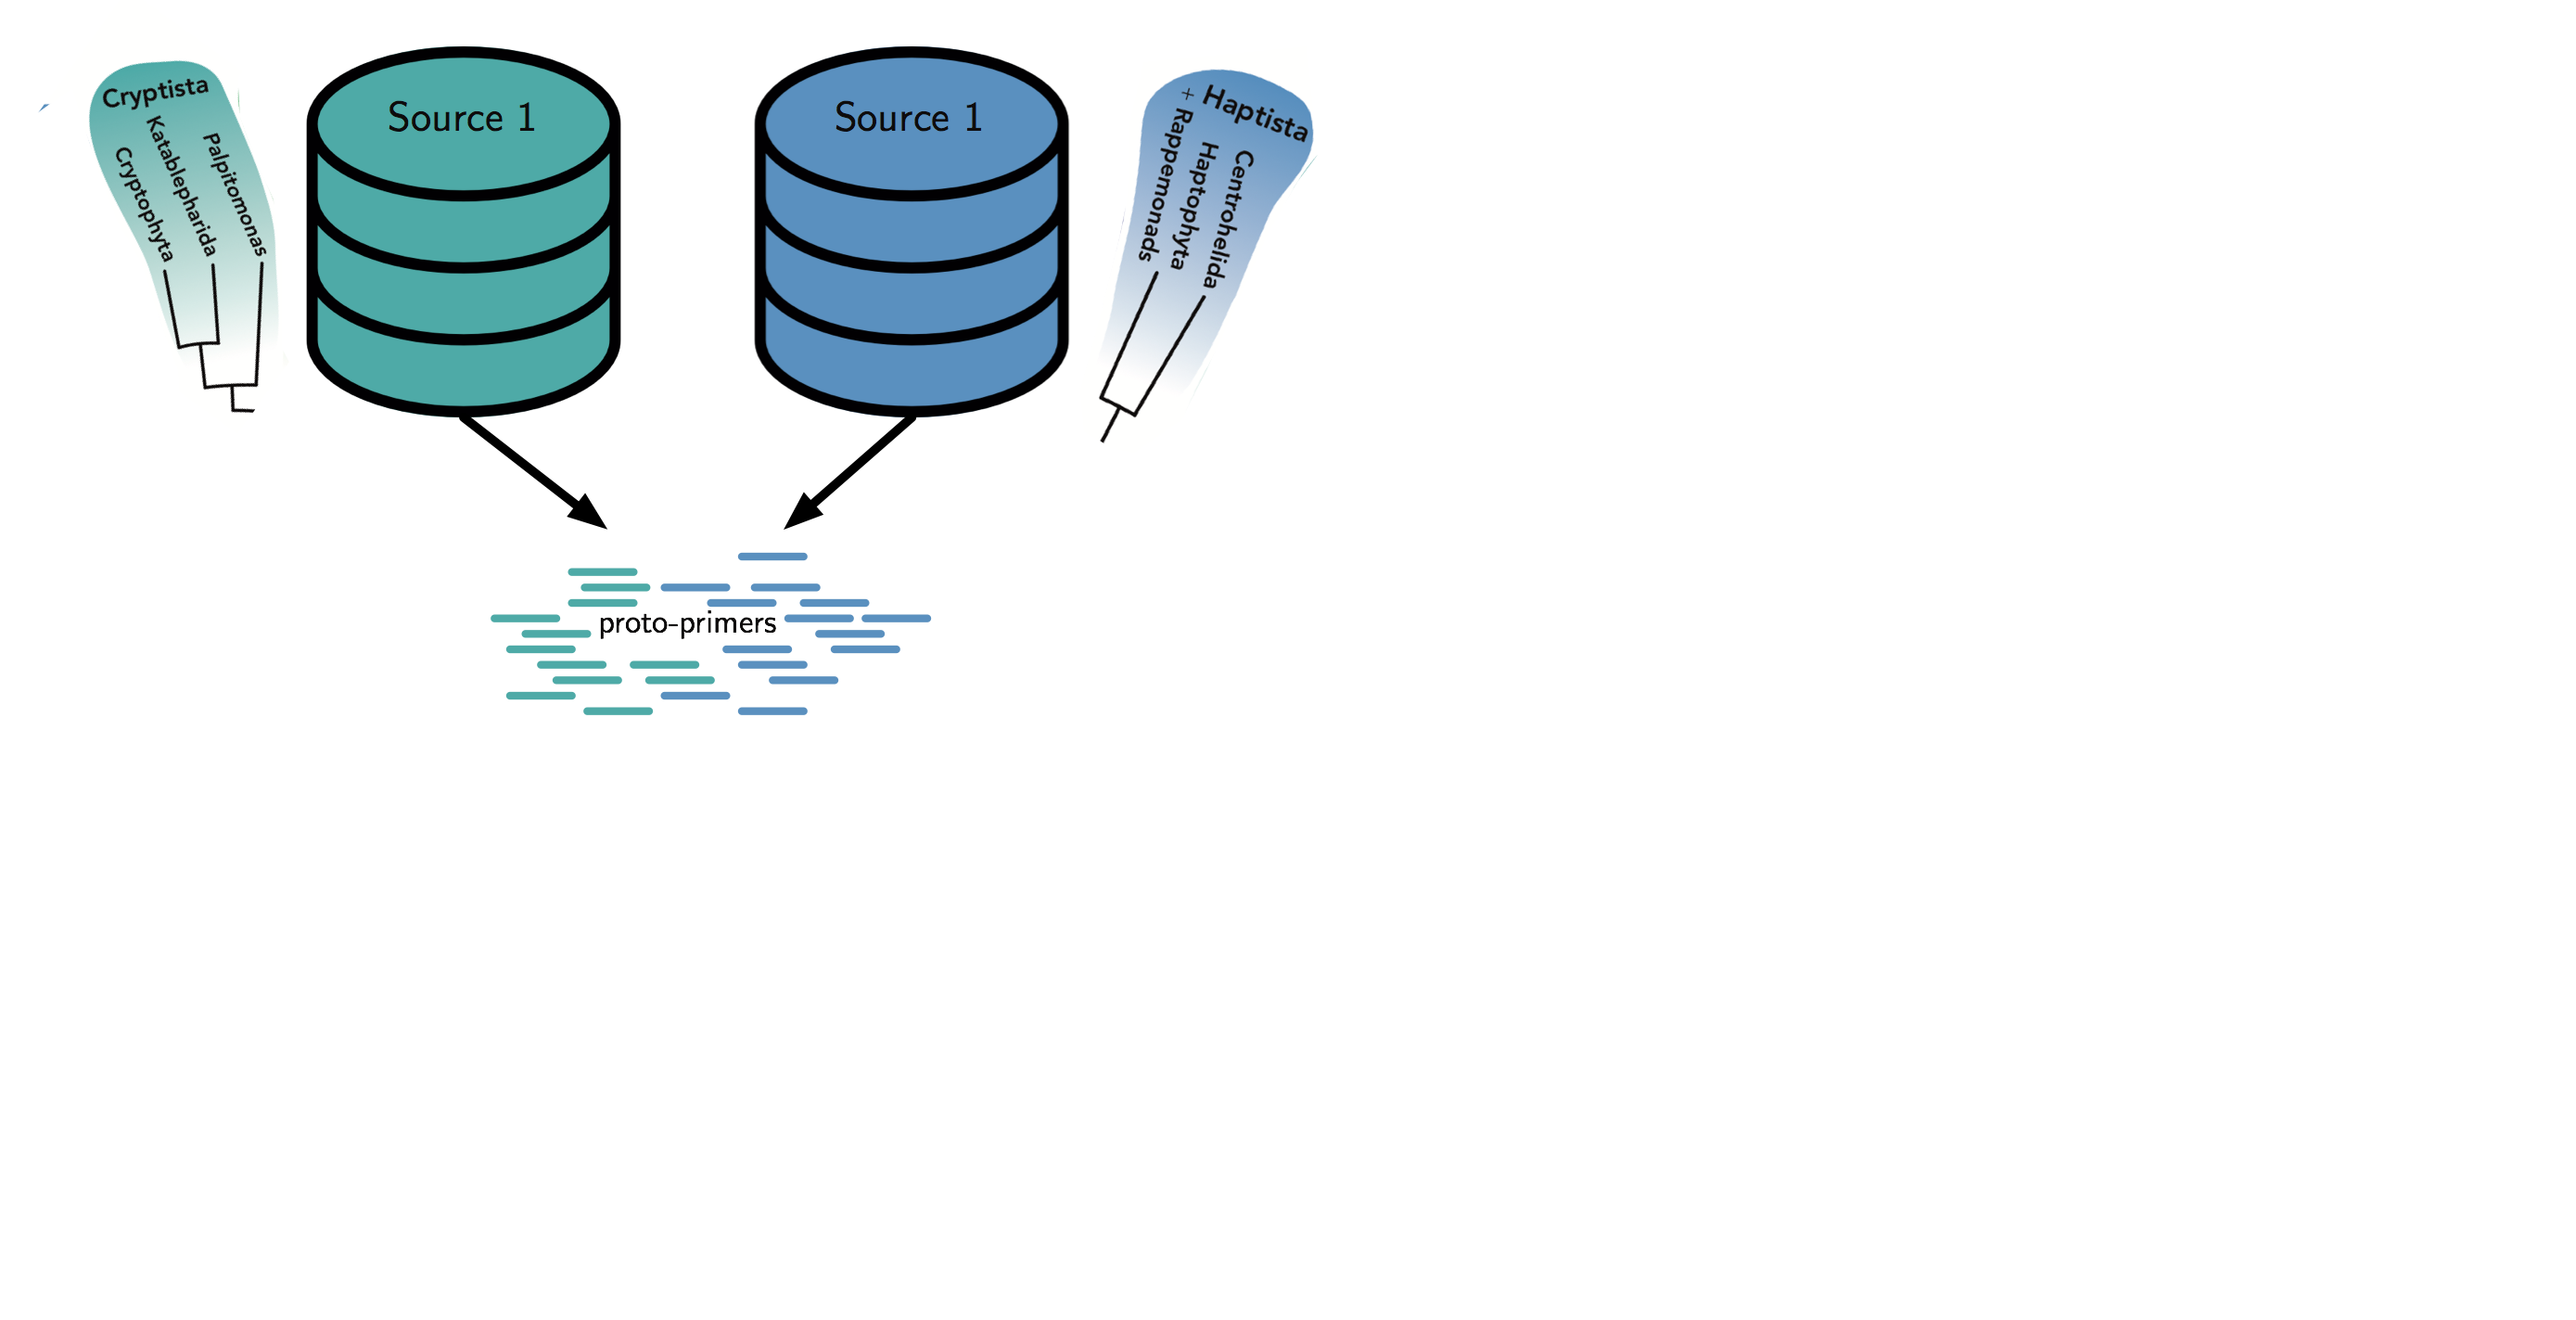
\includegraphics[scale=.4]{DB_protoprimers}
\end{figure}
\end{frame}

\begin{frame}{I Robust Primer Discovery}
\framesubtitle{How to make it computational feasible?}
% \framesubtitle{Primer Search Tool: PriSeT \cite{PriSeTGitHub}}
Avoid multiple sequence alignment computation
%Challenge: amount of primer candidates derivable from database
    \begin{enumerate}
        \item Build FM-index \cite{Ferragina2005} on $T = R_1 \circ  R_2 \circ \cdots \circ R_m$  % combines the Burrows-Wheeler compression algorithm (BW, see Burrows and Wheeler, 1994) and suffix arrays (SAs) to obtain a compressible
        \begin{itemize}
            \item FM-index provides
            \begin{eqnarray*}
            \operatorname{locate} (T, \operatorname{kmer}) &:=& A[l:r]\\
            \operatorname{frequency} (T, k) &:=& [r_i - l_i + 1]_{i\in [1:|T|]}
            \end{eqnarray*}
            with $l_i$, $r_i$ denoting the ranges for k-mer $T[i:i+k-1]$
        \end{itemize}
        \item Lookup k-mers with minimal frequency threshold
    \end{enumerate}
    % TODO: illustration
% \vskip0pt plus 1filll
\flushdown
\rule{\textwidth}{.8pt} 
{\footnotesize
\begin{description}
    \item[$R_i$] reference sequence
    \item[$k$] target length for proto-primer
    \item[kmer] = proto-primer
    \item[$A$] suffix array derived from text $T$ 
\end{description}
}
\end{frame}

\begin{frame}{I Robust Primer Discovery}
\framesubtitle{How to make it computational feasible?}
% \framesubtitle{Primer Search Tool: PriSeT \cite{PriSeTGitHub}}
Primer fitness test
\begin{enumerate}
    \item Two-bit encoding scheme %(Fig. \ref{TKMerID})
    \item<2> Bit-parallelism %(Fig. \ref{bitparallel_CG})
\end{enumerate}
\only<1>{
    \begin{figure}
        \includegraphics[scale=.3]{TKMerID}
        \caption{K-mer compression scheme.}\label{TKMerID}
    \end{figure}
}
\only<2>{
    \setcounter{figure}{3}
    \begin{figure}
        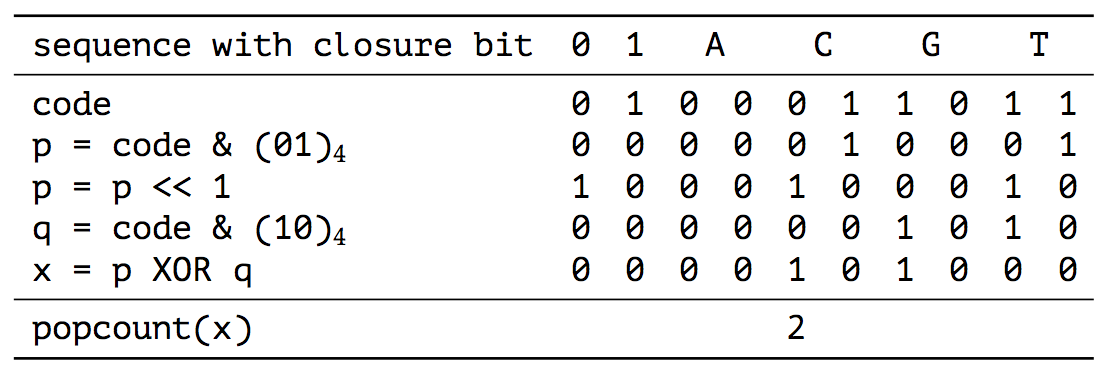
\includegraphics[scale=.5]{bitparallel_CG}
        \caption{Bit-parallelized counting of CG.}\label{bitparallel_CG}
    \end{figure}
}
\flushdown
Presented techniques implemented in PriSeT \cite{PriSeTGitHub}.
\end{frame}

\begin{frame}{I Robust Primer Discovery}
\framesubtitle{Evaluation on Plankton Dataset: Library}
\begin{figure}
    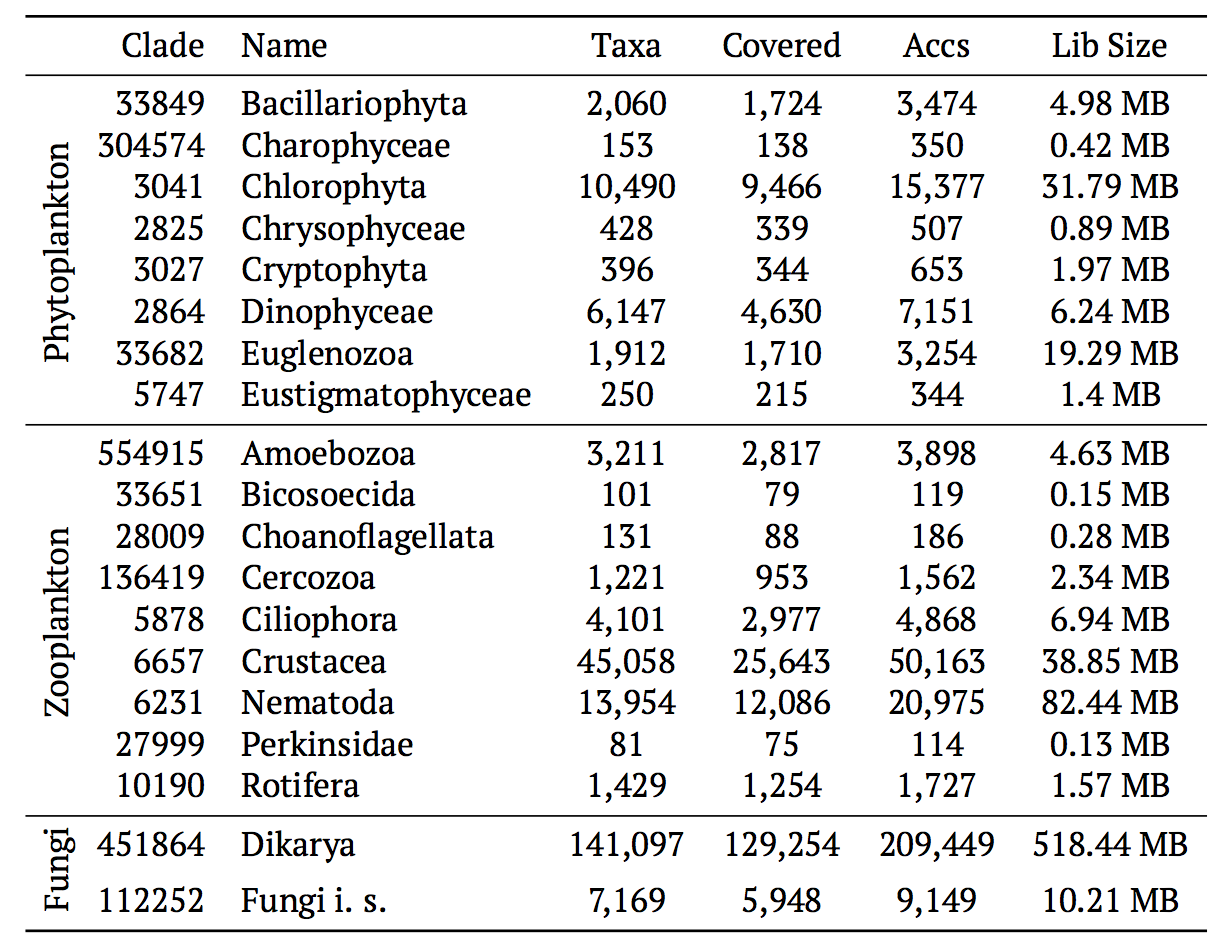
\includegraphics[scale=.38]{plankton_data}
    \caption{Reference sequences sampled from plankton taxa as found in GenBank's nt dataset.}
\end{figure}
% \hfill
\end{frame}

\begin{frame}{I Robust Primer Discovery}
\framesubtitle{Evaluation on Plankton Dataset: comparison of proto-primer}
\begin{figure}\centering
    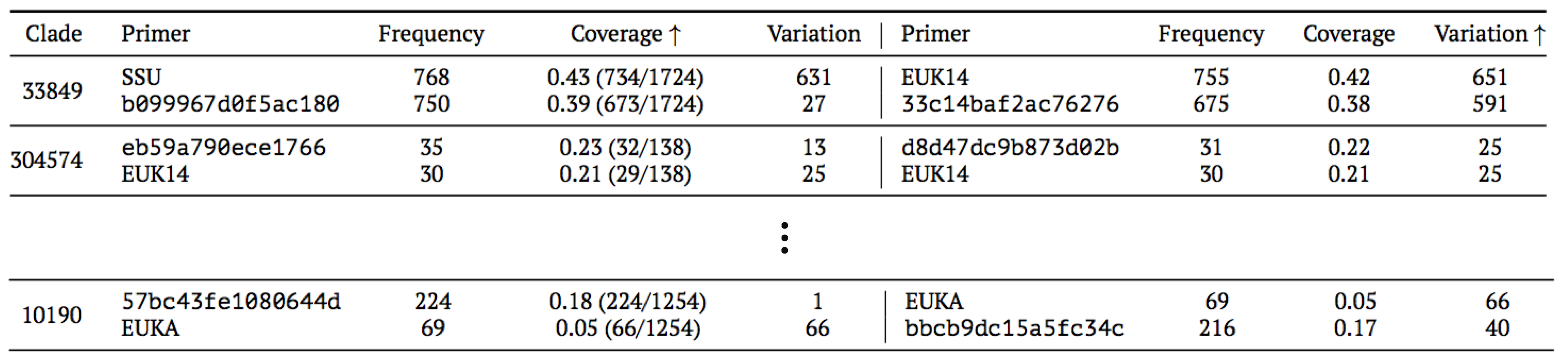
\includegraphics[scale=.47]{denovo_plankton}
    \caption{Excerpt from table of computed proto-primers (16-digits) compared to published primer pairs (SSU, EUK14, EUKA). Coverage: number of sequences covered. Variation: number of unique amplicon.}
\end{figure}
Results: at least one new primer pair identified by PriSeT
\begin{itemize}
    \item Ranking by coverage: for 11 / 19 clades %, PriSeT identifies at least one new primer pair with a higher coverage rate % than the published primers
% \hfill
    \item Ranking by amplicon variation: for 7 / 19 clades %, PriSeT found at least one more or equally performant primer pair
\end{itemize}
% given that the rSSU is already a well studied and exploited region, is not too bad
\end{frame}

\begin{frame}{I Robust Primer Discovery}
\framesubtitle{Evaluation on Plankton Dataset: Runtime of proto-primer generation}
\begin{figure}\centering

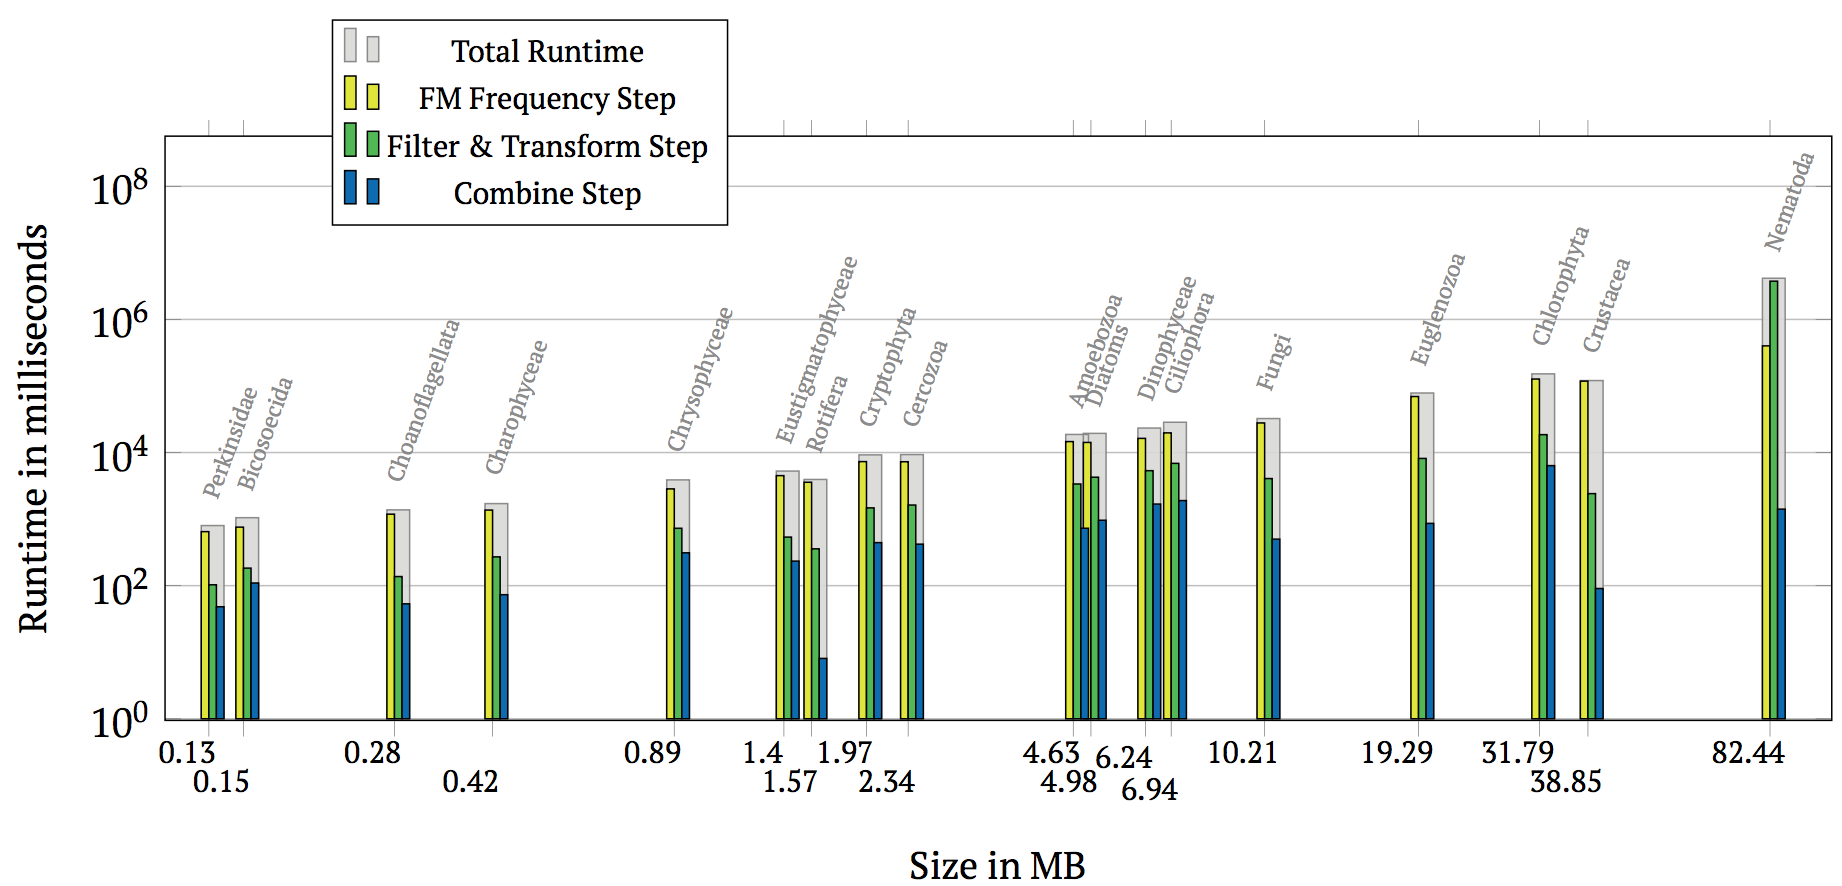
\includegraphics[scale=.36]{plankton_runtime}
    \caption{Runtimes for plankton clades vary from about 1 sec (Perkinsidae) to 15 min (Nematoda).}
\end{figure}

\end{frame}

% Demonstration on over-exploited ribosomal region: found unreported primer pairs \cite{PriSeT2021}

\begin{frame}{Motivation: Lake Monitoring Project}
\framesubtitle{Desiderium for Ongoing Protocol Enhancement II}
\begin{enumerate}[II]
    \item Structured digitalization of protocols, past studies
    \begin{itemize}
        \item Allow for meta-analyses 
        % Example: Where is the data set used in study X?
        % most effective primer for species X in terms of OTU size?
        \item Shorten ramp-up period of new hires % researchers, interns, students, visiting researchers
        \item Improve reproducability of analyses
    \end{itemize}
   
\end{enumerate}
\begin{figure}\centering
    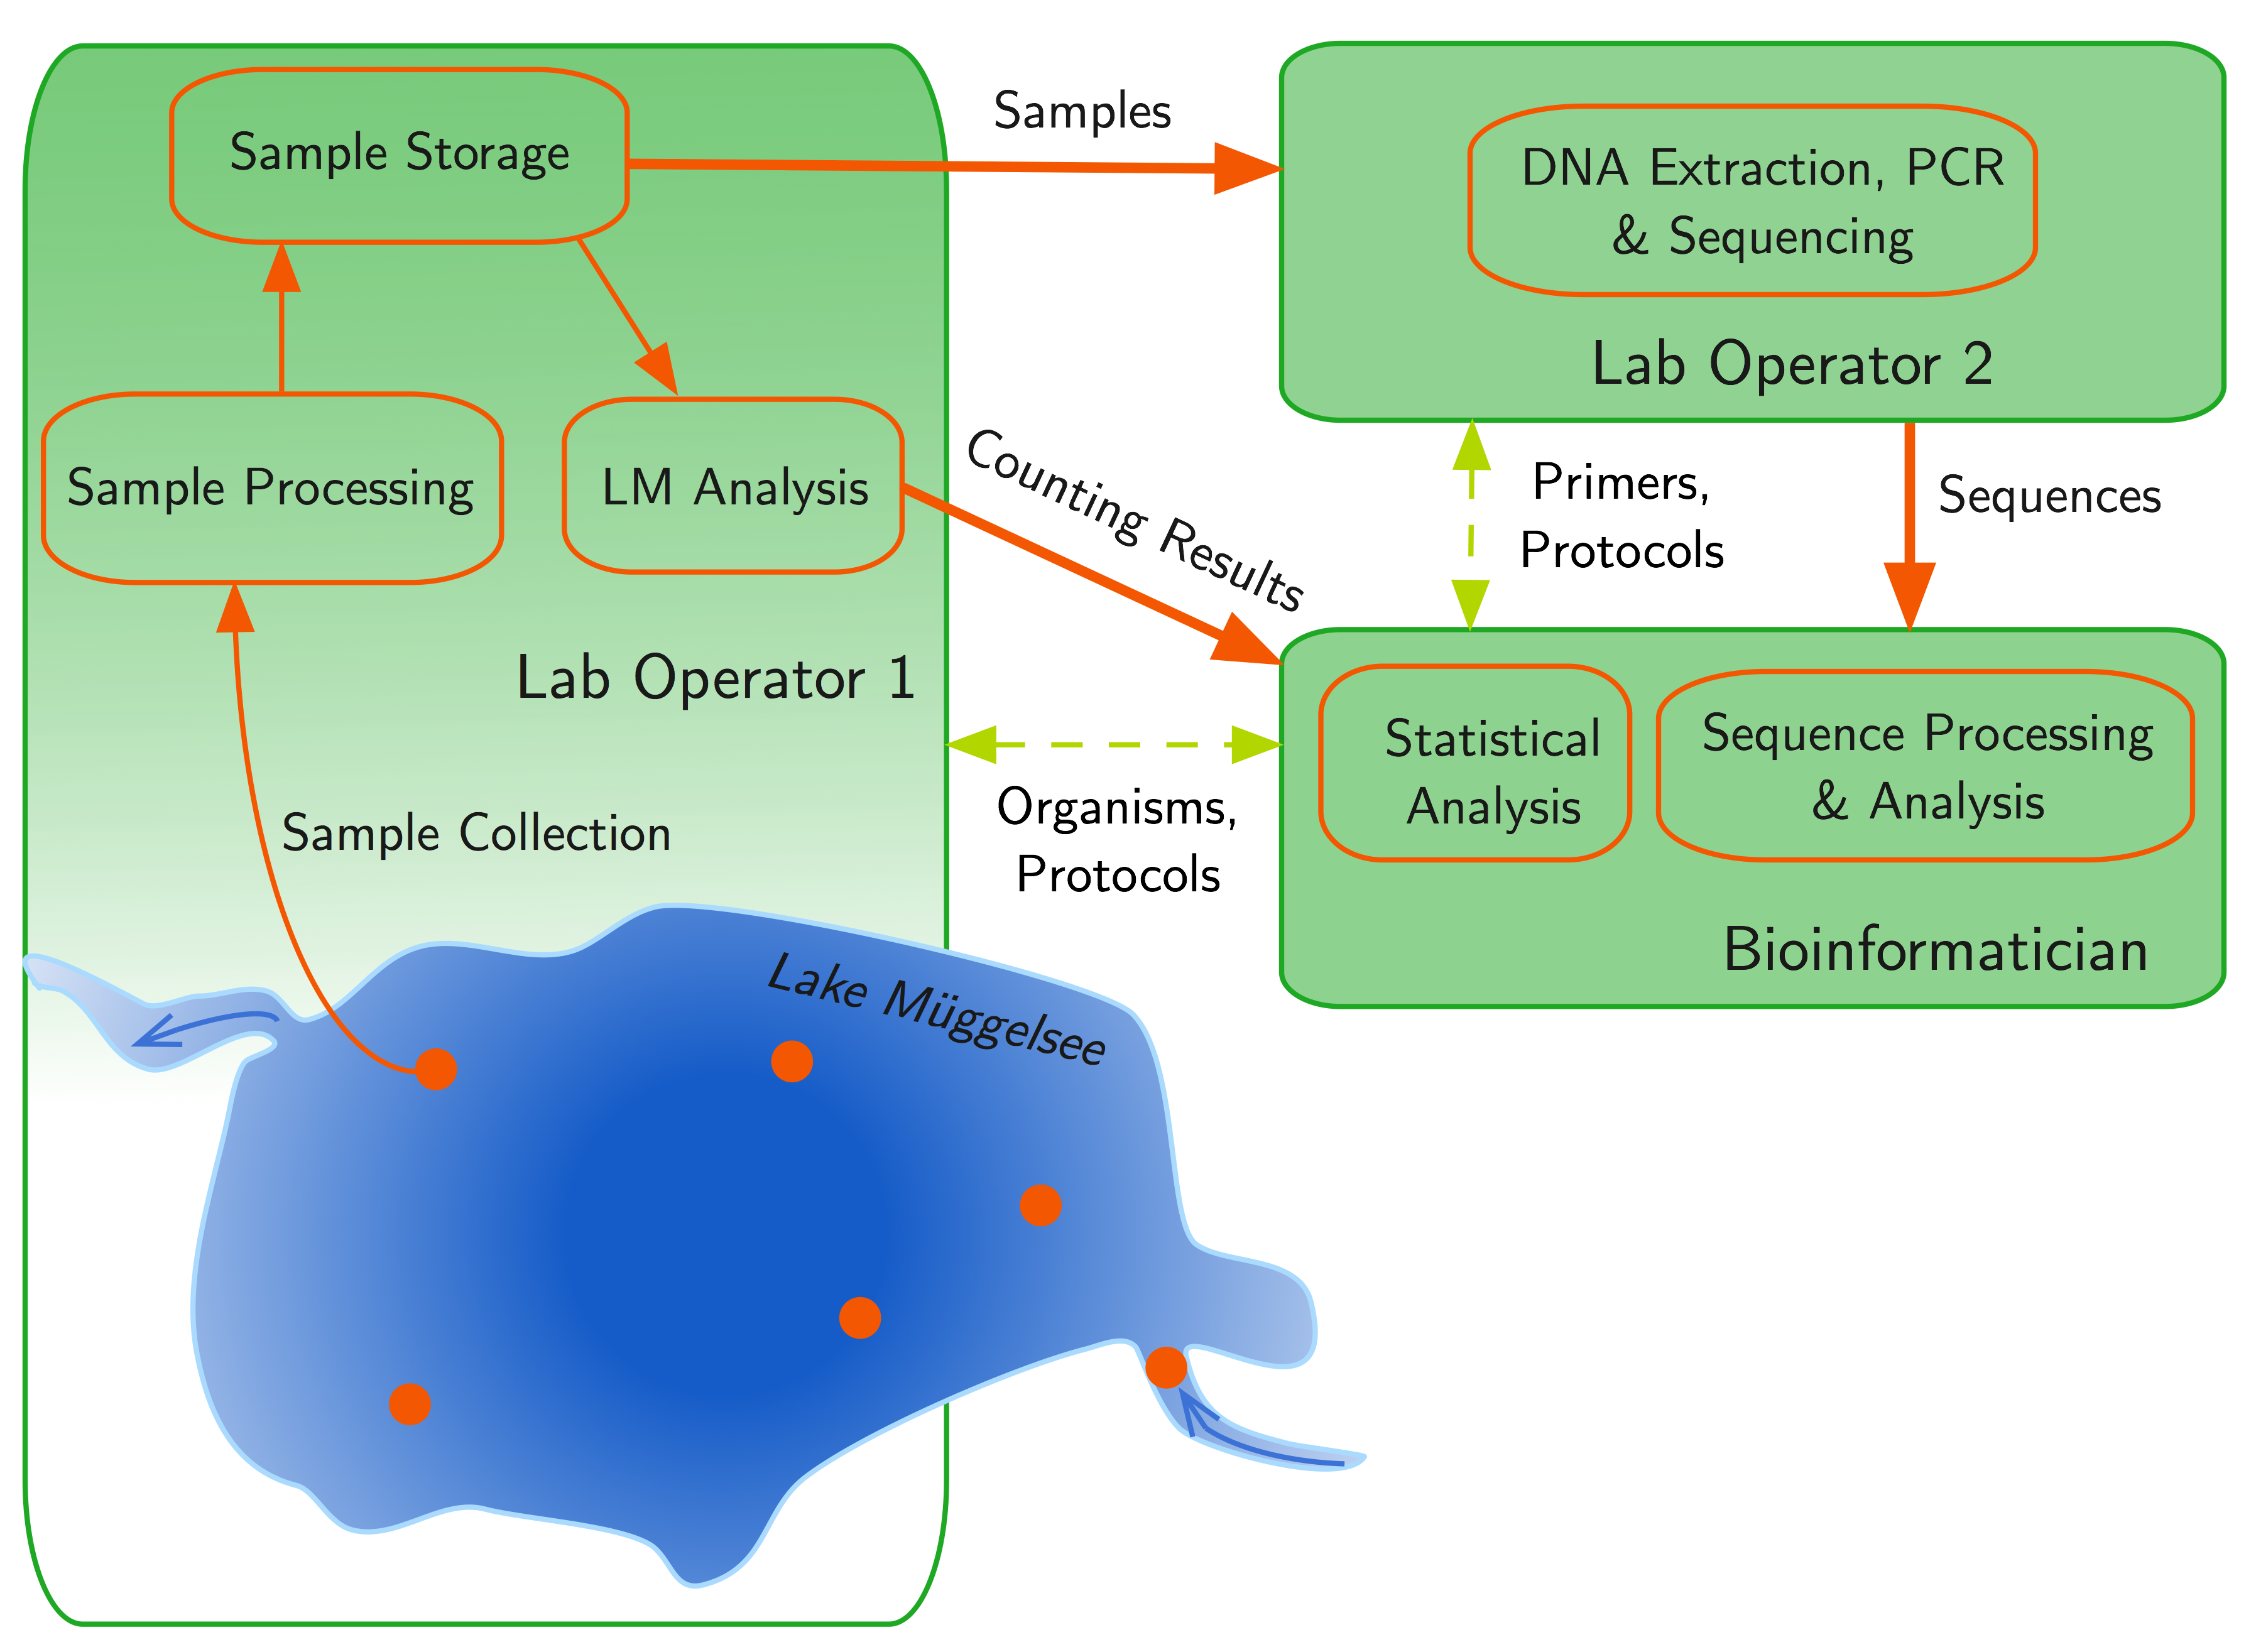
\includegraphics[scale=.45]{DB_flow}
    \caption{Data transfer between lab operators and bioinformaticians.}
\end{figure}
% Concretely:
%     * Problem: short stay of researchers, disjoint, splattered results, and the often quoted repeatability of experiments, each researcher has its own tool set, goes through the same evolution, sometimes rebuild pipelines to see if their results match -> slows down the pace
% * new types of analyses could be conducted if experimental setups, results are consolidated into a single scheme
% *  significant example here!
% * see DB schema
% * repeatability: serialisation of analysis pipelines
  
\end{frame}


\begin{frame}{II Database Schema}\framesubtitle{Data Consolidation and Querying}
  \begin{figure}\centering
    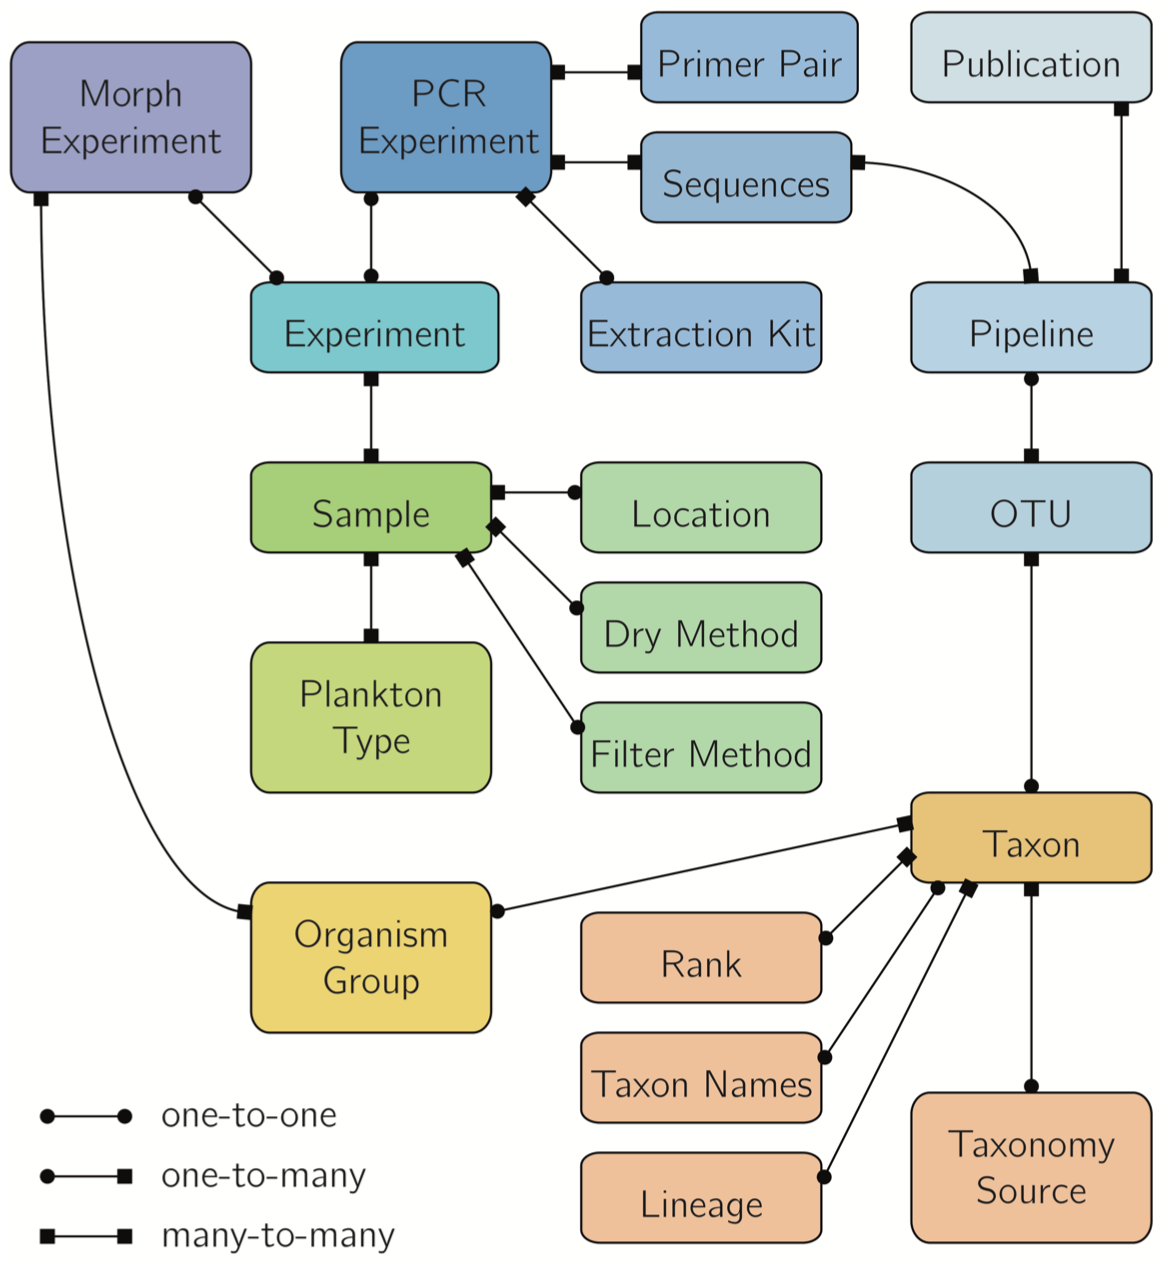
\includegraphics[scale=.3]{DB_schema}
    \caption{Database schema \cite{PlanktonDB}}
    \end{figure}
\end{frame}


%----------- REFERENCES  -------------
%----------- No editing in references section ----------
%----------- edit only in References.bib ----------
	\begin{frame}[allowframebreaks]
		\justifying
		\frametitle{List of References}
		\printbibliography
	\end{frame}
%--------- THANK YOU Text --------------------------
	\begin{frame}
		\centering
		\begin{block}
			\scshape
				\begin{center}
					\large\emph{Thanks to} % I want to express my gratitude
				\end{center}
				\begin{itemize}
				    \item \underline{Commission}: Knut Reinert, Michael T. Monaghan, Katharina Jahn, Sandro Andreotti
				    \item \underline{Bioinformatics Group}: SeqAn Team
				    \item \underline{BeGenDiv}: Tatiana Semenova-Nelson, Camilla Mazzoni, Felix
				    \item \underline{IGB}: Rita Adrian, Justyna Wollinska, Ursula Newen, any many more
				\end{itemize}
		\end{block}
    \nocite{Burki2020, PriSeT2021}
	\end{frame}
%----------------------------------------------------
\end{document}
